
\documentclass[12pt,a4paper,oneside]{book}
%\usepackage[latin1]{inputenc}
\usepackage{amsmath}
\usepackage{amsfonts}
\usepackage{amssymb}
\usepackage[spanish]{babel}
\usepackage[utf8]{inputenc}
\usepackage[spanish]{babel}
\usepackage[graphicx]{realboxes}
\usepackage{wrapfig}
\usepackage{fancyhdr}
\usepackage[hidelinks]{hyperref}
\usepackage{datatool}
\usepackage[acronym]{glossaries}
\usepackage{makeidx}
\usepackage{multirow}
\usepackage{multicol}
\usepackage{colortbl}
\usepackage{cite}
\usepackage{ieeetrantools}
\usepackage{float}
\makeindex
\pagestyle{fancy}

\makeglossaries % este comando debe estar en el preámbulo

\begin{document}
\renewcommand{\glossaryname}{Glosario}

\renewcommand\listtablename{\'Indice de Tablas}
%\listtablename

\renewcommand{\tablename}{Tabla}
\renewcommand{\acronymname}{Acr\'onimos y s\'imbolos}
\renewcommand{\bibname}{Referencias bibliogr\'aficas}
%\glsaddall
\frontmatter
\vspace*{-3cm}
\begin{figure}[h]
\leavevmode
\begin{minipage}{\textwidth}
\begin{center}
%\includegraphics[scale=0.5]{./logofpune}
\end{center}
\end{minipage}
\end{figure}

\thispagestyle{empty}

{\bf
\begin{center}
\large
\vspace*{-1 cm}\Large \textsc{Universidad Nacional del Este.} \\
\Large \textsc{Facultad Politécnica.} \\
\vspace*{0.5 cm}\hrule
\end{center}
}

\vspace*{-0.5 cm}
\begin{figure}[htb]
\begin{center}

\includegraphics[scale = .6]{./portada_y_ficha_catalografica/logo.png}

\end{center}
\end{figure}


\vspace{3 cm}
{
\noindent
\begin{center}
\huge \bf Red de monitoreo de calidad del aire en Alto Paraná.
\end{center}
}


\vspace{6 cm}

\begin{center}
{\textbf{\Large Rafael Nicolás Garcia Britos.}\\[5mm]
\textbf{\Large Camila Belén Guerrero Mercado.}\\[5mm]
\vspace{1 cm}
\textbf{Año \the\year.}}
\end{center}

\bstctlcite{IEEEexample:BSTcontrol} % cambia "and" por "y" en bibliografía

\vspace*{-3cm}
\begin{figure}[h]
\leavevmode
\begin{minipage}{\textwidth}
\begin{center}
%\includegraphics[scale=0.5]{./logofpune}
\end{center}
\end{minipage}
\end{figure}

\thispagestyle{empty}

{\bf
\begin{center}
\large
\vspace*{-1 cm}\Large \textsc{Universidad Nacional del Este.} \\
\Large \textsc{Facultad Politécnica.} \\
\vspace*{0.5 cm}\hrule
\vspace*{0.5 cm}\Large Carrera Ingeniería de Sistemas.\\
\vspace*{0 cm}\Large Cátedra Trabajo Final de Grado II.\\
\end{center}
}

\vspace{3.5 cm}
{
\noindent
\begin{center}
\huge \bf Red de monitoreo de calidad del aire en Alto Paraná.
\end{center}
}


\vspace{0.5 cm}
{ 

Por: \textbf{\Large Rafael Nicolás Garcia Britos.}\\[5mm]
\hspace*{1.5cm}\textbf{\Large Camila Belén Guerrero Mercado.}

\vspace*{.5 cm}
Profesor Orientador: \textbf{\large Ing. Daisy Kang.}
}%\\[6mm]
\vspace*{0.5 cm}\\
Trabajo final de grado presentado a la Facultad Politécnica de la Universidad Nacional del Este como parte de los requisitos para optar al título de Ingeniero de Sistemas con Énfasis en Sistemas Empotrados.

\vspace{4.0cm}
\begin{center}
{\large {\bf Ciudad del Este, Alto Paraná. Paraguay.}\\[6mm]
Diciembre 2023}
\end{center}
%\newpage
% ********** Ficha Catalográfica
\newpage \normalsize
\thispagestyle{empty}
\begin{center} 
\begin{tabular}{c} 
  FICHA CATALOGRÁFICA \\
  BIBLIOTECA DE LA FACULTAD POLITÉCNICA \\
  DE LA UNIVERSIDAD NACIONAL DEL ESTE \\
\end{tabular} %\smallskip
\vspace{0.3cm}

\begin{tabular}{|l|} \hline %  \hspace{1.5cm}
\\
Garcia Britos, Rafael Nicolas, 1996.\\
Guerrero Mercado, Camila Belén, 1996.\\
Red de monitoreo de calidad del aire en Alto Paraná. \\
Ciudad del Este, Alto Paraná. Año: 2023.\\
Páginas: $<$cantidad de páginas$>$.\\ 
\\
Orientador: Ing. Daisy Kang. \\

Área de estudio: Ingeniería de Software, Ingeniería de Sistemas. \\
Carrera: Ingeniería de Sistemas con Énfasis \\
en sistemas empotrados. \\
Titulación: $<$denominación del (de la) profesional$>$. \\

Trabajo Final de Grado. Universidad Nacional del Este, \\
Facultad Politécnica.\\
\\ \\

Descriptores: 1. Calidad del aire, 2. Contaminación del aire, \\
\hspace{2cm} 3. Sensores, 4. LoraWAN, 5. Internet de las Cosas.\\
Air Quality Monitoring Network in Alto Paraná. \\
Key words: 1. Air Quality, 2. Air Pollution \\
\hspace{2cm} 3. Sensors,  4. LoraWAN, 5. Internet of Things.\\
\hline
\end{tabular}
\end{center}


% ********** Dedicatoria
%\vspace*{8in}
%\newpage
\thispagestyle{empty}

Yo, Daisy Isabel Kang Cardozo, documento de identidad No. 4.202.423, Profesor Orientador del TFG titulado ``\textit{Red de monitoreo de calidad del aire en Alto Paraná}'', de los alumnos Rafael Nicolás Garcia Britos, documento de identidad No. 4.379.480, y Camila Belén Guerrero Mercado, documento de identidad No. 4.227.704, de la carrera Ingeniería de Sistemas de la Facultad Politécnica de la Universidad Nacional del Este; certifico que el mencionado Trabajo Final de Grado ha sido realizado por dichos alumnos, de lo cual doy fe y en mi opinión reúne las condiciones para su presentación y defensa ante la Mesa Examinadora designada por la institución.

\begin{flushright}Ciudad del Este, \rule{1cm}{0.4pt} de \rule{2cm}{0.4pt} de 2023\end{flushright}
\vspace{0.7cm}
	
\hspace{7cm}\rule{6cm}{0.4pt}
\begin{flushright}
Ing. Daysi Kang
\end{flushright}
		
\vspace{1.6cm}
Nosotros, los miembros de la Mesa Examinadora del Trabajo Final de Grado titulado ``$<$\textit{Red de monitoreo de calidad del aire en Alto Paraná}'', de la carrera Ingeniería de Sistemas de la Facultad Politécnica de la Universidad Nacional del Este, hacemos constar que el citado trabajo ha sido evaluado en fondo y forma por esta Mesa, la que por \rule{4cm}{0.4pt} ha resuelto asignar la calificación \rule{2cm}{0.4pt}

\begin{flushright}Ciudad del Este, \rule{1cm}{0.4pt} de \rule{2cm}{0.4pt} de 2023 \end{flushright}

\vspace{.5cm}
\hspace{2.2cm}\rule{7cm}{0.4pt}\\
\hspace*{3cm} Profesor \rule{4.5cm}{0.4pt}\\
\hspace*{2.8cm} Presidente de la Mesa Examinadora
\vspace{.7cm}

\hspace*{-0.4cm}\rule{6cm}{0.4pt}\hspace{1.15cm}\rule{6cm}{0.4pt}\\
\vspace{.3cm}
Profesor \rule{4.5cm}{0.4pt}		\hspace{.9cm}Profesor \rule{4.5cm}{0.4pt}\\
Miembro de la Mesa Examinadora\hspace{1cm}Miembro de la Mesa Examinadora
%\normalsize
%% ********** Dedicatória - Back Page
%\newpage 
%\thispagestyle{plain} 
%\null

% ********** Dedicatoria
%\vspace*{8in}
%\newpage
\thispagestyle{empty}
\null\vfill
\begin{flushright}
  {\large{\textit{Escribir aquí la dedicatoria.\\
  Su extensión no debería exceder de una página.}}}
\end{flushright} %\normalsize
%% ********** Dedicatória - Back Page
%\newpage 
%\thispagestyle{plain} 
%\null

\thispagestyle{empty}
\null\vfill

$<${\large \textit{Escribir aquí los agradecimientos.}}$>$

$<${\large \textit{Su extensión no debería exceder de una página.}}$>$

\thispagestyle{empty}
\null\vfill
\begin{flushright}

$<${\large \textit{Escribir aquí el epígrafe (frase u oración favorita).}}$>$

$<${\large \textit{Su extensión no debería exceder de una página.}}$>$

\end{flushright}

\thispagestyle{empty}
\begin{center}
\begin{LARGE}
\textbf{Resumen}
\end{LARGE}
\end{center}
\begin{quotation}

Ante la creciente preocupación por la calidad del aire en el Alto Paraná y la ausencia de una red de monitoreo adecuada, se ha desarrollado una red de monitoreo ambiental para medir contaminantes clave como el dióxido de nitrógeno (NO2), dióxido de carbono (CO2), ozono (O3) y material particulado (PM). Se integran también sensores de temperatura y humedad, factores críticos que afectan la química de algunos contaminantes del aire.

El núcleo de esta red de monitoreo consiste en el microcontrolador ESP32 de Heltec, seleccionado por su robustez y capacidad de procesamiento. Este microcontrolador tiene integrado un módulo LoRaWAN que hace la transmisión de datos a través de The Things Network (TTN), aprovechando su eficiencia en el consumo de energía y su capacidad para operar en redes de sensores distribuidos. El sistema se alimenta mediante un convertidor de corriente continua a corriente alterna, asegurando una operación continua y fiable.

El sistema propuesto ofrece una solución robusta para los desafíos de la calidad del aire en Alto Paraná. Proporcionando datos precisos y actualizados sobre los contaminantes atmosféricos y las condiciones ambientales, el proyecto apoya esfuerzos de concienciación, regulación y mitigación de la contaminación. Además, establece una base para futuras investigaciones y medidas de sostenibilidad ambiental en la región.

Este trabajo detalla el diseño y la implementación técnica del sistema de monitoreo y destaca la importancia de la accesibilidad y la comprensión de los datos ambientales. La capacidad de visualizar y analizar estos datos es fundamental para impulsar cambios positivos y proteger la salud y el bienestar de las poblaciones locales, así como la integridad del ecosistema de Alto Paraná.

\vspace*{0.5cm}

\noindent {\bf Descriptores:} 1. Red de Monitoreo, 2. Calidad del Aire, 
3. Contaminantes del aire, 4. Sensores.

\end{quotation}

\addcontentsline{toc}{chapter}{Resumen}
\thispagestyle{empty}
\begin{center}
\begin{LARGE}
\textbf{Abstract}
\end{LARGE}
\end{center}

\begin{quotation}
To address the growing concern about air quality in Alto Paraná and the lack of a monitoring network, we have developed an environmental monitoring network that measures key pollutants such as nitrogen dioxide (NO2), carbon dioxide ( CO2), ozone (O3) and particulate matter (PM). In addition, temperature and humidity sensors are integrated since they are critical factors that affect the chemistry of some air pollutants.

The heart of our monitoring network is made up of the Heltec ESP32 microcontroller, which has been selected for its robustness, processing capacity with the integrated LoRaWAN module. The latter allows long-range, low-power wireless communication, ideal for deploying a sensor network in large urban areas. The system is powered by a direct current to alternating current converter, guaranteeing continuous and reliable operation.

The proposed system offers a robust solution to address air quality challenges in Alto Paraná. By providing accurate and up-to-date data on air pollutants and environmental conditions, the project supports pollution awareness, regulation and mitigation efforts. Furthermore, it establishes a basis for future research and measures of environmental sustainability in the region.

This work not only details the design and technical implementation of the monitoring system but also highlights the importance of accessibility and understanding of environmental data. The ability to visualize and analyze this data is essential to drive positive changes and protect the health and well-being of local populations, as well as the integrity of the Alto Paraná ecosystem.

\vspace*{0.5cm}

\noindent {\bf Key words:} 1. Monitoring network, 2. Air quality
,3. Air pollutants, 4. Sensors.
\end{quotation}

\addcontentsline{toc}{chapter}{Abstract}
\tableofcontents
\listoffigures
\addcontentsline{toc}{chapter}{\'Indice de figuras}
\listoftables
\addcontentsline{toc}{chapter}{\'Indice de tablas}
\printglossary[type=\acronymtype] % imprime solo la lista de acrónimos
%\cleardoublepage
\addcontentsline{toc}{chapter}{Acr\'onimos y s\'imbolos}
\mainmatter
\fancyhead{}
\fancyfoot{}
\lhead{Introducción}
\cfoot{\thepage}

\chapter{Introducción}

En América Latina, la vigilancia de la calidad del aire representa una tarea pendiente de vital importancia. La región enfrenta un crecimiento económico y urbano acelerado, lo que conlleva un aumento en la emisión de contaminantes atmosféricos. Sin embargo, la infraestructura para monitorear y gestionar estos contaminantes es a menudo insuficiente. Este déficit es particularmente evidente en Paraguay, donde la expansión industrial y la urbanización continúan sin un seguimiento ambiental adecuado.

La calidad del aire que respiramos está directamente relacionada con nuestra salud y bienestar, así como con la salud de los ecosistemas que nos sostienen. La medición precisa de los contaminantes atmosféricos es fundamental para comprender y mitigar los impactos negativos de la contaminación. El propósito de este proyecto es desarrollar una red de monitoreo que utilice tecnología avanzada para medir concentraciones de contaminantes atmosféricos específicos, tales como el dióxido de nitrógeno (NO2), dióxido de carbono (CO2), ozono (O3) y material particulado (PM). Además, se monitorean variables ambientales como la temperatura y la humedad, que juegan un papel crucial en la interpretación de los datos de calidad del aire. La relevancia de este monitoreo radica en el hecho de que estos contaminantes tienen implicaciones directas en la salud humana. Este sistema no solo tiene como objetivo recopilar datos precisos y en tiempo real, sino que también proporciona una interfaz de visualización de estos datos, permitiendo una interpretación clara y oportuna para el usuario final.



%Este capítulo típicamente realiza la presentación de todo el Trabajo Final de Grado (TFG), excepto por las conclusiones que no deben ser adelantadas aquí. Se considera este capítulo como el inicio de la parte textual del informe del trabajo, toda la redacción preliminar a la introducción corresponde así a la parte pretextual del mismo. Debería incluir, generalmente en este orden \cite{sampieri}.


\section{Motivación}
La inspiración para este proyecto surge de una preocupación profunda por el bienestar de las comunidades, especialmente en la región de Alto Paraná. La motivación principal es doble: por un lado, existe una necesidad urgente de abordar la escasez de datos ambientales en América Latina y, por otro, un deseo de contribuir a la mejora de la salud pública y la preservación del medio ambiente a través de la aplicación de tecnologías de monitoreo avanzadas.

En América Latina, y en Paraguay en particular, el monitoreo de la calidad del aire ha sido históricamente limitado, lo que ha llevado a una falta de conciencia y comprensión sobre sus impactos. Esta carencia de información impide la capacidad de los responsables políticos y la sociedad civil para tomar decisiones informadas que protejan la salud pública y respondan a los desafíos ambientales. La región de Alto Paraná, con su dinámica mezcla de urbanización, industria y áreas naturales, representa un microcosmos de los desafíos ambientales que enfrenta el país.

Este libro tiene como objetivo llenar ese vacío informativo, proporcionando no solo datos valiosos sobre la calidad del aire sino también una metodología replicable para el monitoreo ambiental. La motivación se extiende a empoderar a las comunidades locales con el conocimiento y las herramientas necesarias para abogar por un ambiente más limpio y saludable. Además, se busca inspirar a otros investigadores y profesionales a desarrollar y aplicar soluciones innovadoras en sus propias regiones.

Finalmente, la motivación para este libro es también personal y académica. Representa la culminación de un proyecto de grado que no solo tiene la intención de cumplir con un requisito académico sino también de dejar una huella positiva en la sociedad, contribuyendo a un futuro más sostenible para Paraguay y estableciendo un precedente para la acción ambiental en toda América Latina.

\section{Definición del problema}

El problema central que este trabajo busca abordar es la significativa falta de infraestructura y datos sobre la calidad del aire en Alto Paraná, Paraguay, y, por extensión, en muchas regiones de América Latina. A pesar de la creciente industrialización y urbanización, que conllevan un aumento en la emisión de contaminantes atmosféricos, existe una notable ausencia de sistemas de monitoreo ambiental capaces de proporcionar datos fiables y en tiempo real. Esta carencia de información impide una evaluación precisa de la exposición a la contaminación del aire y sus efectos en la salud pública y el medio ambiente.

La región de Alto Paraná, conocida por su importante contribución al PIB nacional a través de la agricultura, la industria y la energía hidroeléctrica, enfrenta el desafío de equilibrar el desarrollo económico con la sostenibilidad ambiental. La contaminación del aire plantea riesgos para la salud humana, incluyendo enfermedades respiratorias y cardiovasculares, y afecta negativamente a la biodiversidad local.

Además, las condiciones climáticas de Alto Paraná, que incluyen altas temperaturas y niveles variables de humedad, pueden exacerbar la concentración y los efectos de los contaminantes. Sin embargo, la falta de un sistema de monitoreo adecuado ha dejado un vacío en la comprensión y gestión de estos problemas ambientales.

Este trabajo final de grado se propone diseñar e implementar un sistema de monitoreo de calidad del aire que no solo aborde la escasez de datos, sino que también sirva como modelo para la implementación de tecnologías similares en otras regiones con desafíos parecidos. La ausencia de un monitoreo efectivo es un obstáculo significativo para la formulación de políticas de salud y ambientales basadas en evidencia, donde este proyecto busca proporcionar las herramientas necesarias para superar este obstáculo.



Definición del problema: \textit {Necesidad de Red de monitoreo de calidad del aire en Alto Paraná.}

\section{Objetivos}
\subsection{Objetivo general}
Desarrollar prototipo de Red de monitoreo de calidad del aire en Alto Paraná.


\subsection{Objetivos específicos}

\begin{enumerate}
\item Conocer los parámetros permisibles de la calidad del aire.
\item Conocer las herramientas físicas para la medición de partículas.
\item Diseñar dispositivos para el monitoreo de los contaminantes de la calidad del aire, como:
\begin{enumerate}
\item Ozono(O3)
\item Monóxido de Carbono(CO)
\item Dióxido de Nitrógeno(NO2)
\item Material Particulado de 2.5 micras
\item Material Particulado de 10 micras
\end{enumerate}
\item Implementar una red de nodos capaces de recolectar variables de calidad del aire.
\item Generar un algoritmo para la comunicación entre servidor y nodos.
\item Almacenar y gestionar los datos obtenidos de la calidad del aire.
\item Monitorear en tiempo real variables recolectadas por los nodos.
\end{enumerate} \pagebreak

\section{Hipótesis}

Se hipotetiza que la implementación de una Red de Monitoreo de Calidad del Aire en Alto Paraná proporcionará datos significativos sobre los niveles de contaminantes atmosféricos. Estos datos facilitarán la toma de decisiones informadas y mejorarán la gestión de políticas de salud y medio ambiente. Se espera que esta red de monitoreo contribuya a una mejor comprensión de los patrones de contaminación y sus impactos, lo que a su vez permitirá desarrollar estrategias más efectivas para abordar los problemas relacionados con la calidad del aire en la región.


\section{Justificación}

La necesidad de monitorear la calidad del aire en Alto Paraná se justifica por varias razones críticas que tienen implicaciones directas en la salud pública, la sostenibilidad ambiental y el desarrollo económico de la región.

Salud Pública: La exposición a contaminantes atmosféricos está vinculada a una serie de problemas de salud, incluyendo enfermedades respiratorias agudas y crónicas, enfermedades cardiovasculares y un aumento en la mortalidad. La implementación de un sistema de monitoreo permitirá identificar y cuantificar estos contaminantes, contribuyendo significativamente a la prevención de riesgos para la salud de la población.

Sostenibilidad Ambiental: Alto Paraná alberga una biodiversidad rica y ecosistemas sensibles que están en riesgo debido a la contaminación. Un sistema de monitoreo proporcionará datos esenciales para la conservación de estos recursos naturales y para el desarrollo de estrategias de mitigación de impactos ambientales.

Desarrollo Económico: La región de Alto Paraná es un motor económico para Paraguay, y su desarrollo sostenible es clave para el futuro del país. La calidad del aire tiene un impacto directo en la calidad de vida y en la capacidad de la región para atraer inversiones y turismo. Por lo tanto, un sistema de monitoreo es esencial para equilibrar el crecimiento económico con la protección ambiental.

Marco Regulatorio: La falta de datos concretos sobre la calidad del aire ha limitado la capacidad del gobierno para desarrollar y aplicar regulaciones efectivas. Este proyecto proporcionará la información necesaria para formular políticas basadas en evidencia y para cumplir con los estándares internacionales de calidad del aire.

Innovación Tecnológica: La adopción de tecnologías avanzadas para el monitoreo ambiental en Paraguay puede servir como un modelo para otras regiones en América Latina que enfrentan desafíos similares, promoviendo así la innovación y el liderazgo tecnológico en la región.

\section{Delimitación del alcance del trabajo.}

El presente trabajo final de grado se enfoca en el diseño, implementación y evaluación de un sistema de monitoreo de calidad del aire en la región de Alto Paraná. El alcance del proyecto está delimitado por los siguientes parámetros:

Geográfico: El estudio se circunscribe a la región de Alto Paraná, sin incluir comparaciones directas con otras regiones de Paraguay o análisis en profundidad de zonas urbanas y rurales diferenciadas dentro de la región.

Temporal: La recopilación de datos y la evaluación del sistema se llevarán a cabo durante un periodo específico, que será determinado por la duración del proyecto de grado.

Metodológico: El proyecto se limitará a la implementación de tecnología de monitoreo y no abarcará intervenciones para reducir los niveles de contaminación. Además, el análisis se centrará en la viabilidad técnica y la precisión de los datos, sin entrar en el diseño de políticas públicas basadas en los resultados.

Impacto: Mientras que se discutirá el potencial impacto del sistema de monitoreo en la formulación de políticas y la salud pública, el alcance del trabajo no incluirá la implementación real de políticas ni el seguimiento de cambios en la salud pública tras la introducción del sistema.

Esta delimitación asegura que el trabajo se mantenga enfocado y manejable, permitiendo una profundización en los aspectos clave del diseño e implementación del sistema de monitoreo de calidad del aire, y proporcionando una base sólida para futuras investigaciones que puedan expandir el alcance del estudio inicial.



\section{Descripción de los contenidos por capítulo.} 
	\item \textbf{Capítulo 1. Introducción: }Este capítulo establecerá el contexto del proyecto, resaltando la importancia de monitorear la calidad del aire en Alto Paraná. Se expondrán la motivación, la justificación, la hipótesis y los objetivos del estudio, así como la delimitación del alcance del trabajo. Se ofrecerá una visión general del problema de la calidad del aire en la región y cómo este proyecto busca abordarlo.
 
	\item  \textbf{Capítulo 2. Marco Teórico: }En este capítulo se proporcionará una revisión exhaustiva de la literatura sobre la calidad del aire y sus impactos en la salud y el medio ambiente. Se explorarán los conceptos fundamentales de la contaminación atmosférica, los tipos de contaminantes y sus fuentes, así como los estándares internacionales de calidad del aire.
 
	\item  \textbf{Capítulo 3. Herramientas Utilizadas: }En este capítulo se describirán en detalle las herramientas tecnológicas empleadas en el proyecto. Se incluirá una descripción del hardware y del software. Se explicará la selección de estas herramientas, su configuración y su integración en el sistema de monitoreo.\gls{anpr}.
 
	\item  \textbf{Capítulo 4: Resultados: }En este capítulo se presentará los datos recogidos durante el periodo de estudio. Se mostrarán las mediciones de los contaminantes atmosféricos y las condiciones ambientales, y se ilustrará cómo estos datos se visualizan a través de una interfaz. Se incluirán gráficos, tablas y otras representaciones visuales para facilitar la comprensión de los resultados.
 
	\item  \textbf{Capítulo 5: Discusión: }En este capítulo se interpretará los resultados obtenidos, comparándolos con la hipótesis y los objetivos del estudio. Se evaluará la eficacia del sistema de monitoreo y se discutirán las implicaciones de los hallazgos para la salud pública y la política ambiental. Este capítulo también abordará las limitaciones del estudio, sugerencias para investigaciones futuras y recomendaciones basadas en los resultados del proyecto.
 


\fancyhead{}
\fancyfoot{}
\newtheorem{teorema}{Teorema}
\cfoot{\thepage}

\lhead{Conceptos fundamentales y antecedentes}
%\rhead{\today}
%\rfoot{\thepage}

\chapter{Conceptos fundamentales y antecedentes}
\section{Conceptos fundamentales}

\subsection{Medición}
La medición de la calidad del aire se realiza mediante el uso de sensores de partículas, los cuales son calibrados por el fabricante para garantizar la precisión de los datos. Estos sensores capturan información específica sobre la concentración de contaminantes atmosféricos en el aire. Los datos recogidos por los sensores son leídos y procesados por una microcomputadora, que desempeña un papel crucial en la transmisión de esta información a un servidor con acceso a Internet.

En el servidor, los datos son analizados y procesados para calcular el denominado "índice de calidad del aire" (AQI, por sus siglas en inglés). Este índice permite clasificar la calidad del aire en seis categorías, que van desde "Buena" hasta "Peligrosa". Esta clasificación se basa en el grado de contaminación y sigue las directrices establecidas por la Agencia de Protección Medioambiental de los Estados Unidos (EPA). El AQI es una herramienta valiosa para informar al público sobre la calidad del aire en tiempo real y para tomar decisiones relacionadas con la salud y el medio ambiente.

\subsection{Sensores}

Un sensor es un dispositivo diseñado para detectar y medir una magnitud física o química, conocida como variable de instrumentación, y convertirla en una señal eléctrica que puede ser procesada, almacenada o transmitida según la finalidad definida por el usuario. En el contexto de la medición de la calidad del aire, los sensores juegan un papel crucial al proporcionar datos precisos y en tiempo real sobre diversos contaminantes atmosféricos.

Los sensores pueden funcionar de diversas maneras, dependiendo de su aplicación específica:
\begin{itemize}
\item Algunos sensores proporcionan una lectura directa en la unidad de interés, lo que facilita una interpretación rápida y sencilla de los datos.

\item Otros sensores se conectan a instrumentos que leen la señal y la traducen a la unidad deseada, permitiendo una mayor flexibilidad en la presentación de los datos.

\item También existen sensores que se conectan a dispositivos capaces de almacenar la señal para su procesamiento posterior, lo que es esencial para el análisis a largo plazo y la tendencia de los datos.
\end{itemize}
Los sensores se clasifican según su aplicación, el tipo de señal de salida que generan, o más comúnmente, según la variable física o química que miden. Por ejemplo, en el monitoreo de la calidad del aire, se utilizan sensores específicos para medir concentraciones de contaminantes como el dióxido de nitrógeno (NO2), dióxido de carbono (CO2), ozono (O3) y material particulado (PM).

Con el avance de la tecnología electrónica, los sensores no solo se limitan a traducir cantidades físicas en visualizaciones más simples, sino que también se han integrado en una amplia gama de campos tecnológicos, desde aplicaciones industriales hasta dispositivos de consumo.

\subsection{Red de Sensores}
Una red de sensores es un conjunto de dispositivos distribuidos espacialmente diseñados para medir variables ambientales y físicas, y comunicar esta información a través de nodos interconectados. Estas redes son fundamentales para recopilar datos a gran escala, permitiendo un monitoreo detallado y en tiempo real de condiciones específicas.

\subsection{Ventajas:}

\begin{itemize}
\item Monitoreo en Tiempo Real: Las redes de sensores proporcionan datos actualizados continuamente, esenciales para la detección oportuna de niveles peligrosos de contaminantes y para la respuesta rápida a eventos ambientales.

\item Cobertura Espacial Amplia: Permiten el monitoreo de grandes áreas, superando las limitaciones de las estaciones de monitoreo fijas y aisladas, y proporcionando una visión más completa de la calidad del aire en una región.

\item Resolución de Datos Alta: La capacidad de desplegar múltiples sensores aumenta la resolución de los datos, permitiendo una comprensión más detallada de las variaciones locales en la calidad del aire.

\item Flexibilidad y Escalabilidad: La capacidad de desplegar múltiples sensores aumenta la resolución de los datos, permitiendo una comprensión más detallada de las variaciones locales en la calidad del aire.
\end{itemize}


\subsection{Desventajas:}
\begin{itemize}
\item Mantenimiento y Calibración: : Los sensores requieren mantenimiento regular y calibración para mantener la precisión de los datos, lo que puede ser logísticamente desafiante.

\item Limitaciones de los Sensores de Bajo Costo:  Aunque son más accesibles, pueden ofrecer menor precisión y fiabilidad que los equipos de monitoreo más sofisticados.

\item Vida Útil de la Batería: Los sensores inalámbricos dependen de baterías que necesitan ser reemplazadas o recargadas periódicamente.

\item Interferencias y Pérdida de Datos: Las condiciones ambientales adversas o la interferencia electromagnética pueden afectar la transmisión de datos.

\item Gestión de Datos:  La gran cantidad de datos generados requiere sistemas avanzados para su procesamiento, análisis y almacenamiento.
\end{itemize}

\subsection{Calidad del Aire}
La calidad del aire se refiere a la condición del aire en nuestro entorno y cómo esa condición afecta a la salud de los seres vivos y al medio ambiente. Se mide generalmente en términos de concentraciones de contaminantes específicos, como partículas en suspensión (PM2.5 y PM10), dióxido de nitrógeno (NO2), dióxido de carbono (CO2), ozono (O3), entre otros. La calidad del aire es un indicador de la salud ambiental y se ha convertido en un área de interés público y científico debido a su impacto directo en la salud humana y los ecosistemas.

Historia y Evolución:
El interés por la calidad del aire surgió con mayor fuerza durante la Revolución Industrial, cuando la quema de carbón en las fábricas y la acumulación de smog se convirtieron en problemas evidentes. Sin embargo, no fue sino hasta mediados del siglo XX, después de episodios graves de contaminación como el Gran Smog de Londres en 1952, que se empezaron a establecer las primeras regulaciones significativas. Desde entonces, la calidad del aire ha sido un área de estudio en constante evolución, con avances en la medición, el análisis y la regulación.

\subsection{Ventajas:}

La monitorización de la calidad del aire ofrece múltiples beneficios, incluyendo la protección de la salud pública mediante la identificación y mitigación de riesgos asociados a la contaminación, la conservación de ecosistemas y biodiversidad, el apoyo al desarrollo de políticas y regulaciones ambientales, y la promoción de la conciencia y educación pública sobre temas de salud y medio ambiente.

\subsection{Desventajas:}

Los desafíos asociados con el monitoreo de la calidad del aire incluyen el costo de implementación y mantenimiento, la complejidad técnica en la interpretación de datos, la variabilidad espacial y temporal que requiere monitoreo constante, y la necesidad de acciones complementarias para abordar efectivamente los problemas de contaminación identificados.

\subsection{Internet de las Cosas}
El concepto de IoT, que emergió en la década de 1990, ha ganado prominencia con el avance en la conectividad a Internet, la miniaturización de la electrónica y el desarrollo de estándares de comunicación. En la actualidad, IoT es un componente esencial de la industria 4.0, desempeñando un papel transformador en varios sectores, incluido el monitoreo ambiental.

\subsection{Ventajas:}

\begin{itemize}
\item Automatización y Control Remoto: Permite la gestión automatizada de dispositivos de monitoreo y la respuesta rápida a los cambios en la calidad del aire.

\item Eficiencia y Precisión: Aumenta la eficiencia en la recopilación de datos y mejora la precisión mediante el uso de múltiples sensores.

\item Análisis Avanzado: Facilita el análisis avanzado de grandes volúmenes de datos ambientales a través de plataformas de IoT que integran inteligencia artificial y aprendizaje automático.
\end{itemize}



\subsection{Desventajas:}

\begin{itemize}
\item Interoperabilidad: La diversidad de dispositivos y plataformas puede llevar a problemas de compatibilidad y estandarización.

\item Dependencia de la Conectividad: La efectividad de IoT está ligada a la disponibilidad y fiabilidad de las conexiones a Internet.

\item Costos de Implementación: Aunque los costos están disminuyendo, la implementación de soluciones de IoT puede requerir una inversión inicial significativa.
\end{itemize}


\section{Antecedentes}

\subsection{Diseño e implementación de un sistema de monitoreo de calidad de aire}
Un antecedente relevante en el campo del monitoreo de la calidad del aire en Paraguay es el proyecto liderado por el Ing. Diego Palacios y financiado por el Consejo Nacional de Ciencia y Tecnología (CONACYT) \cite{sistema_de_monitoreo}. Este proyecto se centró en el diseño y desarrollo de un sistema avanzado para monitorear la calidad del aire, empleando tecnologías de información y comunicación para la recopilación y transmisión automática de datos. Se instalaron estaciones de telemetría en ubicaciones estratégicas, incluyendo la Facultad de Ingeniería de la Universidad Nacional de Asunción y el Centro de Innovación Tecnológica en Luque. Estas estaciones midieron en tiempo real los niveles de varios contaminantes atmosféricos y variables meteorológicas, proporcionando datos valiosos sobre la calidad del aire en la región. Este sistema no solo ha contribuido a la comprensión de la calidad del aire en Paraguay, sino que también ha establecido un modelo para futuros proyectos de monitoreo ambiental en América Latina.

\subsection{Diseño e implementación de un sistema IOT para monitorear calidad de aire}
Un proyecto relevante en el ámbito del monitoreo de calidad del aire utilizando tecnologías IoT es el desarrollado en Bogotá, Colombia, como se documenta en el Repositorio Institucional Séneca de la Universidad de los Andes \cite{Sistema_IOT_monitoreo}. Este proyecto, realizado en 2021, implementó una red de monitoreo de calidad del aire que integraba nodos de monitoreo estáticos y móviles, proporcionando mediciones en tiempo real de varios contaminantes atmosféricos. La comunicación entre los nodos se realizó a través de Wi-Fi y MQTT, con una centralización de datos en Google Cloud Platform (GCP), lo que permitió un análisis detallado y en tiempo real de la calidad del aire en la ciudad.

\subsection{Implementación de una Red de Monitoreo de Material Particulado MP2,5 y MP10 en la Ciudad de Asunción}
En el proyecto \cite{Investigacion_niveles_MP} se trabajó con la integración de las distintas plataformas a nivel hardware como software para la implementación de una red de monitoreo de material particulado MP2.5 y MP10 con el objetivo de lograr la adquisición, procesamiento y transmisión automática de datos y parámetros ambientales (temperatura, humedad relativa y presión atmosférica), obteniendo de esta manera información sobre la concentración de MP en 11 sitios específicos en tiempo real, por un período ininterrumpido de 12 meses. Las mediciones realizadas han demostrado que los valores de MP son influenciados no solo por el tráfico vehicular, sino también por fenómenos naturales y otros de origen antropogénico, como la quema de pastizales, una práctica muy común en el país, sobre todo en la época invernal.

\subsection{Monitoreo de bajo costo de parámetros permisibles de la Calidad de Aire}
En el proyecto \cite{Monitoreo_bajo_costo} se desarrolló un prototipo detector de Material Particulado y gases presentes en el ambiente para determinar la calidad del aire, basado en hardware libre y sensores de bajo costo operativo. Se obtuvo la funcionalidad deseada, lo cual indica la posibilidad de aplicación para realizar controles estimativos de la Calidad Del Aire en distintos puntos de la ciudad.

\fancyhead{}
\fancyfoot{}
\cfoot{\thepage}

\lhead{Herramientas Utilizadas}

\chapter{Herramientas Utilizadas}

Se explicarán las razones fundamentales para optar por las distintas herramientas que incluyen la comunicación entre el servidor y nodo, el protocolo de comunicación,  el lenguaje de programación, base de datos y visualización de los datos recolectados.

\section{LoRaWAN}
Long Range Wide Area Network \cite{gutierrez2011aplicacion} es un protocolo de comunicación y arquitectura de red diseñado para redes inalámbricas de área amplia (WAN) con el objetivo de conectar dispositivos de Internet de las Cosas (IoT) a la internet de manera eficiente, segura y a bajo costo. LoRaWAN utiliza la tecnología de modulación LoRa (Long Range) para permitir la comunicación a largas distancias con un bajo consumo de energía, lo que lo hace ideal para dispositivos IoT que necesitan una vida útil prolongada de la batería.
\begin{itemize}
    \item \textbf{Largo Alcance:} LoRaWAN puede proporcionar cobertura a distancias de varios kilómetros, incluso en áreas urbanas densas o en entornos rurales.
    \item \textbf{Bajo Consumo de Energía:} Los dispositivos conectados a una red LoRaWAN pueden operar durante años con una sola batería, gracias a su eficiencia energética.
    \item \textbf{Seguridad:} Incluye características de seguridad robustas, incluyendo el cifrado de extremo a extremo, la autenticación de dispositivos y la integridad de los datos.
    \item \textbf{Comunicación Bidireccional:} LoRaWAN permite la comunicación bidireccional entre los dispositivos y la red, lo que significa que los dispositivos no solo pueden enviar datos, sino también recibir mensajes.
\end{itemize}

\section{MQTT}
MQTT (Message Queuing Telemetry Transport) \cite{gutierrez2011aplicacion} es un protocolo de mensajería ligero y eficiente diseñado para la comunicación en dispositivos de Internet de las Cosas (IoT). Es particularmente útil en situaciones donde los recursos de red son limitados o los dispositivos tienen capacidades de hardware restringidas. MQTT opera sobre el protocolo TCP/IP y es conocido por su simplicidad y eficiencia en la transmisión de datos.
\begin{itemize}
    \item \textbf{Modelo de Publicación/Suscripción:} utiliza un modelo de publicación/suscripción, donde los dispositivos pueden publicar mensajes en tópicos y suscribirse a tópicos para recibir mensajes. Esto permite una comunicación eficiente y desacoplada entre los dispositivos.
    \item \textbf{Broker MQTT:} El broker es el componente central en una red MQTT. Es responsable de recibir todos los mensajes, filtrarlos, decidir quién está interesado en ellos y luego enviar el mensaje a todos los clientes suscritos.
    \item \textbf{Retención de Mensajes:}MQTT permite retener un mensaje en un tópico para que sea enviado inmediatamente a cualquier cliente que se suscriba a ese tópico.
    \item \textbf{Eficiente:}  MQTT tiene una sobrecarga de protocolo muy baja, lo que lo hace adecuado para redes con ancho de banda limitado.
\end{itemize}

\section{The Things Network}
The Things Network \cite{gutierrez2011aplicacion} es una red global y de código abierto para dispositivos conectados a Internet a través de la tecnología LoRaWAN (Long Range Wide Area Network). 
Proporciona una infraestructura que facilita la conexión de dispositivos IoT a Internet. Los usuarios pueden contribuir a la red conectando sus propios gateways LoRaWAN, que actúan como puentes entre los dispositivos IoT y la red de Internet. Esto crea una red colaborativa y descentralizada que permite a los dispositivos IoT comunicarse y transmitir datos a través de largas distancias.
\begin{itemize}
    \item \textbf{Acceso Abierto:} Cualquiera puede unirse a la red y contribuir conectando un gateway o utilizando la red para conectar dispositivos IoT.
    \item \textbf{Comunidad Activa:} The Things Network cuenta con una comunidad activa de desarrolladores, empresas y entusiastas que contribuyen al crecimiento y mejora de la red.
    \item \textbf{Cobertura Global:} Gracias a la contribución de gateways por parte de usuarios de todo el mundo, The Things Network tiene la capacidad de proporcionar cobertura en una amplia variedad de ubicaciones.
    \item \textbf{Bajo Costo:} Al ser una red de código abierto y colaborativa, los costos asociados con la conexión de dispositivos a la red pueden ser significativamente más bajos en comparación con otras soluciones de conectividad IoT.
\end{itemize}

\section{Amazon Web Services}
Amazon Web Services también conocido como AWS \cite{gutierrez2011aplicacion} es la plataforma de servicios en la nube más popular y ampliamente utilizada en todo el mundo. Proporciona una amplia variedad de servicios de infraestructura y plataforma en la nube donde ofrece más de 200 servicios integrales de centros de datos a nivel global, algunos de ellos son: poder de cómputo, almacenamiento, bases de datos, análisis, redes, herramientas para desarrolladores, herramientas de gestión, IoT (Internet de las Cosas), seguridad y aplicaciones empresariales. Estos servicios ayudan a las empresas a moverse más rápido, escalar y reducir costos de TI(Tecnología de la Información).

\section{AWS IoT Core}
Es un servicio de Amazon Web Services para Internet de las Cosas(IoT) \cite{gutierrez2011aplicacion}.
Este es el servicio central que permite conectar dispositivos IoT a la nube de AWS de forma segura y eficiente. AWS IoT Core soporta millones de dispositivos y billones de mensajes, y puede procesar y enrutar esos mensajes a endpoints de AWS y a otros dispositivos de forma fiable y segura.

\section{Amazon Timestream}
Timestream \cite{gutierrez2011aplicacion} es un servicio de base de datos no relacional(NoSQL) y de series temporales completamente gestionado que está diseñado para escalar de forma eficiente y rentable con el tiempo. Las series temporales son datos que se miden y registran a lo largo del tiempo. Timestream está optimizado para manejar grandes volúmenes de datos de series temporales y proporciona funciones para el procesamiento y análisis de estos datos.
\begin{itemize}
    \item \textbf{Gestión del Tiempo y Retención:} Gestiona automáticamente la retención de datos y mueve los datos entre diferentes niveles de almacenamiento (memoria y disco) en función de políticas definidas por el usuario, optimizando así los costos de almacenamiento en Amazon Web Services.
    \item \textbf{Consultas Eficientes:} El servicio está optimizado para consultas de series temporales, permitiendo a los usuarios realizar análisis complejos y agregaciones de datos de forma rápida y eficiente.
    \item \textbf{Seguridad:} Proporciona funciones de seguridad robustas, incluyendo el cifrado de datos en tránsito y en reposo, y la capacidad de controlar el acceso a los datos mediante políticas de IAM (Identity and Access Management).
 
\end{itemize}

\section{Amazon Grafana}
Amazon Grafana \cite{E_Twahirwa} \cite{knuth} \cite{A_Abd} \cite{A_Evelyn}\cite{A_Rana}\cite{A_Simo}\cite{D_Fermin}\cite{D_Ochoa}\cite{G_Jota}\cite{H_Paz}\cite{H_Siachoque}\cite{LJ_Chen}\cite{M_Rodenas}\cite{OMS}\cite{Y_Simmhan} es una plataforma de análisis y monitoreo de código abierto que es ampliamente utilizada para visualizar y analizar métricas en tiempo real y datos de series temporales. Proporciona herramientas para crear dashboards interactivos y personalizables que permiten a los usuarios visualizar, realizar consultas y entender sus datos de manera más efectiva.
\begin{itemize}
     \item \textbf{Visualización de Datos:} Permite crear una variedad de visualizaciones de datos, incluyendo gráficos de líneas, barras, diagramas de dispersión, y más. Estas visualizaciones ayudan a los usuarios a identificar tendencias, patrones y anomalías en sus datos.
    \item \textbf{Dashboards Personalizables:} Incluye múltiples paneles de visualización, cada uno configurado para mostrar datos específicos. Los dashboards pueden ser compartidos y colaborativos, permitiendo a los equipos trabajar juntos en el análisis de datos.
    \item \textbf{Comunidad y Soporte:} Al ser una herramienta de código abierto, Grafana cuenta con una comunidad activa de usuarios y desarrolladores que contribuyen a su desarrollo y proporcionan soporte.
    \item \textbf{Integración y Extensibilidad:} Se puede integrar con otras herramientas y servicios, y su funcionalidad puede ser extendida a través de plugins y API.
   
\end{itemize}



%Muestra de como insertar una foto
%\begin{figure}[H]
%\begin{minipage}{\textwidth}
%\begin{center}
%\includegraphics[scale=.4]{./capitulo_03/tablazoo}
%\caption{Tabla de modelos de detección previamente entrenados en el conjunto de datos COCO %2017.} \label{fig:tablazoo}
%\end{center}
%\end{minipage}
%\end{figure}


\fancyhead{}
\fancyfoot{}
\cfoot{\thepage}

\lhead{Resultados}

\chapter{Resultados}

Este capítulo presenta el producto del análisis de los datos. Los resultados compendian el eventual tratamiento estadístico que se dio a los datos. Regularmente el orden es: a) análisis descriptivo de los datos, b) análisis inferenciales para responder a las preguntas de investigación y/o probar hipótesis. Según \cite{sampieri}, la American Psychological Association recomienda que primero se describa de manera breve la idea principal que resume los descubrimientos, y posteriormente se los reporten con detalle. Es importante destacar que en este capítulo no se incluyen conclusiones ni sugerencias, tampoco se deben explicar las implicaciones de la investigación. Esto se hace en el capítulo dedicado a la interpretaciones de los resultados, que en esta plantilla se denomina ``Discusión''.

Aquí el investigador se limita a describir sus hallazgos. Una manera útil de hacerlo es mediante elementos como tablas, gráficas, dibujos, diagramas, mapas y figuras generados por el análisis. Son elementos que sirven para organizar datos, de tal manera que el lector los pueda leer y entender las los vínculos entre las variables. Cada uno de dichos elementos debe ir enumerado. Una buena regla para elaborar una tabla es organizarla lógicamente y eliminar la información que pudiera confundir al lector.

Es conveniente brindar una sencilla explicación de las pruebas realizadas y presentar los resultados de la manera más comprensible posible. En este caso las tablas deben ser descritas. Los diagramas, figuras, mapas cognoscitivos, esquemas, matrices y otros elementos gráficos también deben ser numerados según una  lógica secuencial. Se debe observar el principio básico: una buena figura es sencilla, clara y no estorba la continuidad de la lectura. Las tablas, las figuras y los gráficos deben enriquecer el texto; en lugar de duplicarlos, deben comunicar los hechos esenciales, ser coherentes y fáciles de leer y comprender. 

\section{Ejemplos de elementos gráficos}

\textbf{Figuras y Tablas}

Las figuras y tablas deben insertarse en el punto apropiado dentro del texto.

Cada figura debe estar seguida de un epígrafe que la identifique, enumere y describa brevemente. Cada figura debe ser referenciada al menos una vez, a través de su número (Fig. \ref{fig:huella}).

\begin{figure}[H]
\begin{center}

\includegraphics[scale = .5]{./capitulo_04/huella}
\caption{Sensor PMS5003}
\caption{Sensor DHT22}
\caption{Sensor ZE07-CO}
\caption{Sensor ZE14-O3}
\caption{Entorno de desarrollo PlatformIO}
\caption{Terminal de PlatformIO}
\caption{Consola AWS}
\caption{Consola de Helium}
\caption{Consola de The Things Stack}
\caption{Consola de Grafana}


\label{fig:huella}
\end{center}
\end{figure}

Es deseable que las figuras puedan ser interpretadas satisfactoriamente aún cuando sean impresas en blanco y negro. Esto se facilita mucho haciendo uso inteligente de la combinación de colores de forma que se consiga buen contraste entre los colores empleados, máxime si se trata de diagramas, en que a menudo es posible prescindir por completo de otros colores que el blanco y el negro, (como en la figura \ref{fig:termodin}).

\begin{figure}[H]
\begin{center}
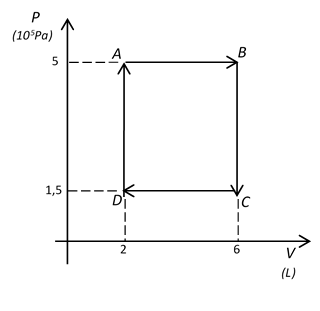
\includegraphics{./capitulo_04/termodin.png}
%\caption{Ejemplificación de diagrama en blanco y negro.}
\label{fig:termodin}
\end{center}
\end{figure}

Las tablas deberían contener datos representativos que sinteticen información significativa del trabajo, evitando mostrar datos intermedios que pudieran dificultar la interpretación del mismo.

Cada tabla debe estar antecedida de un epígrafe que la identifique, enumere y describa brevemente.

Cada tabla debe ser referenciada al menos una vez, a través de su número, de preferencia antes de que aparezca en el documento, como en este caso (tabla \ref{tab:animales}).

\begin{table}[H]
\begin{center}
%\caption{Inventario de animales.}
\label{tab:animales}
\begin{tabular}{||l|l|r||}
\hline
Especie&Sexo&Cantidad\\
\hline
\multirow{2}{*}{palomas}&jóvenes&20\\
&adultas&18\\
\hline
\multirow{2}{*}{conejos}&jóvenes&5\\
&adultos&5\\
\hline
\multirow{2}{*}{gallinas}&jóvenes&50\\
&adultas&50\\
\hline
\multicolumn{2}{||c|}{Total}&148\\
\hline
\end{tabular}
\end{center}
\end{table}

Otro ejemplo de tabla en el cual se observa el empleo de color, además de la combinación de columnas se observa en la tabla \ref{tab:color}

\begin{table}[H]
\begin{center}
\caption{Tabla ICA (Indice de calidad del aire)}
\caption{Tabla de precios}
\caption{Tabla de variables globales}
\caption{Tabla de lecturas NODO 1}
\caption{Tabla de lecturas NODO 2}
\caption{Tabla de lecturas NODO 3}

\label{tab:color}
\begin{tabular}{|c|cccc|}
\hline
\multirow{2}{*}{\cellcolor[rgb]{0.4,0.8,0.5}} &  \multicolumn{4}{>{\cellcolor[rgb]{0.4,0.8,0.9}}c|}{Tamaño de las muestras} \\ 
\cellcolor[rgb]{0.4,0.8,0.5}Edad&\cellcolor[rgb]{0.4,0.8,0.9} San Lorenzo &\cellcolor[rgb]{0.4,0.8,0.9} Asunción &\cellcolor[rgb]{0.4,0.8,0.9} Villarrica &\cellcolor[rgb]{0.4,0.8,0.9} Encarnación \\
\hline
e$<$20 &  93 &  74 &  68 & 87 \\
19$<$e$<$40 &  52 &  48 &  69 & 70 \\
39$<$e$<$60 &  47 &  85 &  81 & 64 \\
59$<$e$<$80 &  28 &  36 &  16 & 23 \\
79$<$e &  9 &  5 &  6 & 12 \\
\hline 
\end{tabular}
\end{center}
\end{table}

Aveces, como en el caso de la tabla \ref{tab:color}, el código se vuelve bastante complejo que resulta engorroso obtener en tiempo razonable la apariencia esperada de la tabla. En esos casos; es posible elaborar la tabla en entorno diferente a Latex; grabarla como imagen png, o jpg, o pdf; e insertarla enmascarada como tabla para ser contada como una de ellas por el contador de tablas: esto se logra con incluir la imagen dentro del entorno ``table'', como se ejemplifica con la tabla \ref{tab:tabla_word} que sigue.

\begin{table}[H]
	\begin{center}
		%\caption{Imagen de tabla, en reemplazo de la tabla anterior.}
		\label{tab:tabla_word}
		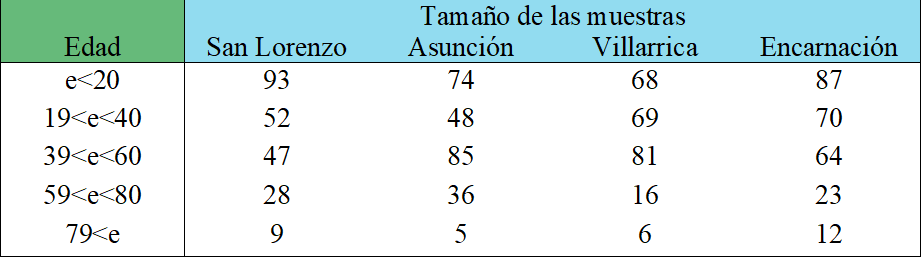
\includegraphics[scale=.65]{./capitulo_04/tabla_word.png}
	\end{center}
\end{table}


\fancyhead{}
\fancyfoot{}
\cfoot{\thepage}

\lhead{Discusión}

\chapter{Discusión}

En este capítulo, que también suele denominarse ``Conclusiones'', se derivan las conclusiones, se explicitan recomendaciones para otros estudios (por ejemplo, sugerir nuevas preguntas, muestras, instrumentos, líneas de investigación, etc.) y se indica lo que sigue y lo que debe hacerse. Se analiza la posibilidad de extender los resultados a una población mayor que la del estudio. Se evalúan las implicaciones, se establece la manera como se respondieron las preguntas de investigación, si se cumplieron o no los objetivos, se relacionan los resultados con los estudios existentes (vincular con el marco teórico y señalar si los resultados coinciden o no con la literatura previa, en qué sí y en qué no). Se reconocen las limitaciones de la investigación, se destaca la importancia y significado de todo el estudio y la forma como encaja en el conocimiento disponible. Se explican los resultados inesperados y cuando no se verificaron las hipótesis es necesario señalar o al menos especular sobre las razones. Recordar que no se deben repetir aquí los resultados sino que se los debe interpretar. La discusión debe redactarse de tal manera que se facilite la toma de decisiones respecto de una teoría, un curso de acción o una problemática. Resumiendo, este capítulo puede ser conceptualmente y dividido en al menos tres secciones, como se ilustra a continuación.

\section{Logros alcanzados}
Descripción de los principales descubrimientos obtenidos como producto de la interpretación de los resultados de la investigación.
\section{Solución del problema de investigación}
Aquí se realiza la discusión propiamente dicha, respondiendo al problema planteado e indicando el nivel de satisfacción de la solución lograda.
\section{Sugerencias para futuras investigaciones}
Todo trabajo de investigación, genera invariablemente como producto colateral, otras interrogantes que suelen ameritar seguir con la investigación. Esto es derivado del caracter abierto, \textit{i.e.}, inacabado, del conocimiento científico. En esta sección se acostumbra hacer referencia a posibles seguimientos de la investigación indicando las interrogantes que conforman nuevos problemas pasibles de ser indagados.   

\backmatter

\cleardoublepage
\addcontentsline{toc}{chapter}{Glosario}
\printglossary

\addcontentsline{toc}{chapter}{Anexos}

\cleardoublepage
\fancyhead{}
\fancyfoot{}
\cfoot{\thepage}

\lhead{Anexo A.}
%\rhead{\today}
%\rfoot{\thepage}

\chapter{Anexo A.}
Los apéndices y anexos resultan útiles para describir con mayor profundidad ciertos materiales, sin distraer la lectura del texto principal del reporte o evitar que rompan con el formato de éste. Algunos ejemplos serían el cuestionario utilizado, un código de programa computacional, análisis estadísticos adicionales, la demostración matemática de un teorema complicado, fotografías testimoniales, etc.



\cleardoublepage
\addcontentsline{toc}{chapter}{Referencias bibliogr\'aficas}

\bibliographystyle{IEEEtran-castellano}
\bibliography{test}
\end{document}

